\chapter{Bounds on \(\mathbf{N}_{\text{patch}}\)}
\label{app:bounds}
\section{2D Green Function Approximation}

Figures~\ref{fig:memoryTime2DGreenFused} and
\ref{fig:memoryTime2DGreenInterleaved} in
Chapter~\ref{chap:results} showed that a patched QTCI (pQTCI) run is advantageous only within a certain window of the patch bond–dimension cap
\(\chi_{\text{patch}}\).   To quantify that window we compare the measured patch count \(\mathcal
N_{\!p}\) with the theoretical bounds (cf. \prettyref{eq:chiPatchBound}) 

\begin{equation}
    \Np
    \;<\;
    \begin{cases}
      \displaystyle\chi^{2}/\chip^{2}, & \text{(memory)},\\[6pt]
      \displaystyle\chi^{3}/(d\,\chip^{3}), & \text{(time)},
    \end{cases}
  \label{eq:chiPatchBoundApp}
\end{equation}
where \(\chi\) is the rank of the corresponding single–TT (standard QTCI)
approximation at the same discretisation parameters \((\mR,\tau)\).

For the pQTCI approximated function \(\operatorname{Re}G(\bk)\) [\prettyref{eq:2DGreen}] we plot \(\Np-\bigl(\chi^{2}/\chi_{\text{patch}}^{2}\bigr)\) and
\(\Np-\bigl[\chi^{3}/(d\,\chip^{3})\bigr]\) for
selected \((\delta)\) values and index unfoldings.   
Negative values mean that the bound is not correctly satified.

\begin{figure}
    \centering
    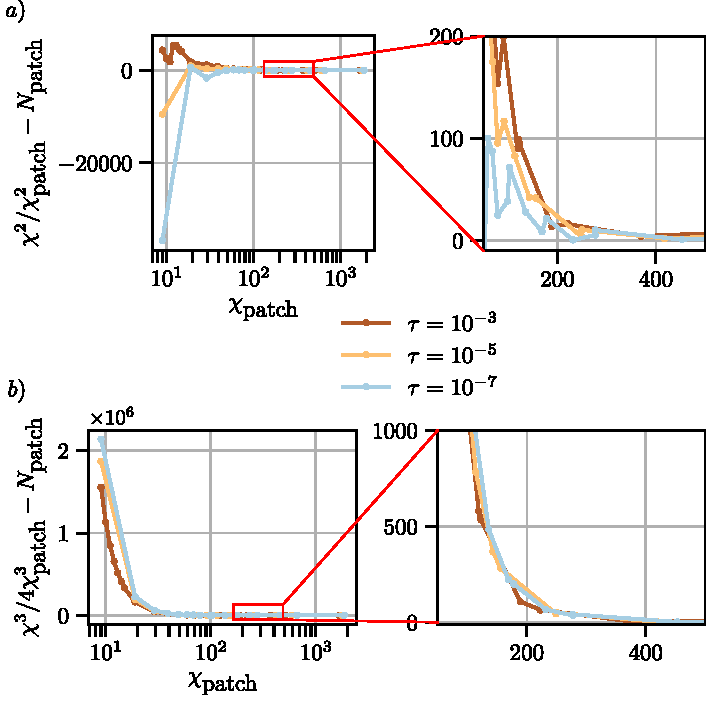
\includegraphics{figures/2DGreenMemoryTimeBoundFused.pdf}
    \caption{\textbf{Fused ordering, \(\delta=10^{-3}\).}
    Difference between the actual patch count \(\Np\) and the memory (a) and run–time (b) bounds of \prettyref{eq:chiPatchBoundApp}.
    Negative bars indicate that the bound is not respected.}
    \label{fig:memoryBound2GreenFused}
\end{figure}

\begin{figure}
    \centering
    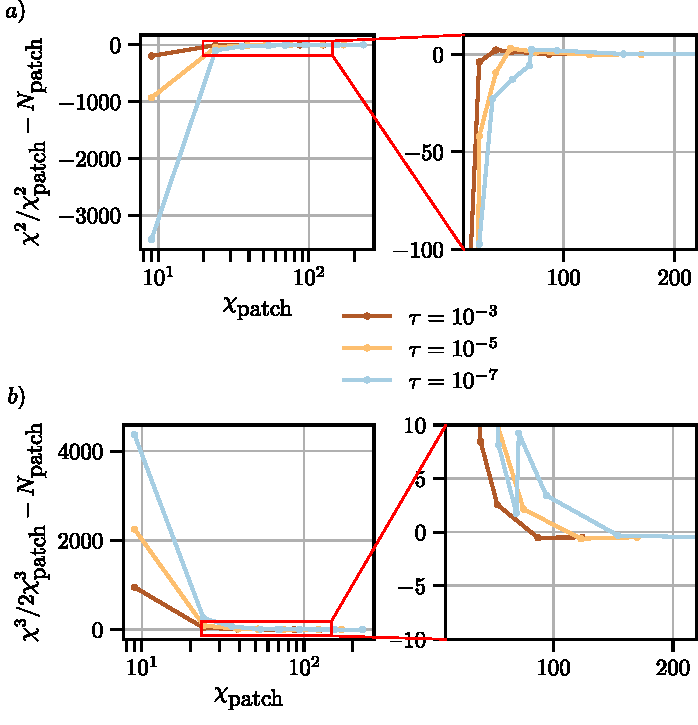
\includegraphics{figures/2DGreenMemoryTimeMemoryBoundInterleaved.pdf}
    \caption{\textbf{Interleaved ordering, \(\delta=10^{-1}\).}
    Same analysis as Fig.~\ref{fig:memoryBound2GreenFused}.
    Here pQTCI tends to \emph{violate} the bounds more often because \(\operatorname{Re}G(\bk)\) is already smooth and the algorithm over–patches the domain.}
    \label{fig:memoryBound2GreenInterleaved}
\end{figure}

Several trends emerge:

\begin{itemize}
  \item For sharp spectral lines (\(\delta=10^{-3}\), fused ordering,
        Fig.~\ref{fig:memoryBound2GreenFused}) the bounds are comfortably
        met in the optimum \(\chi_{\text{patch}}\) range, explaining the
        clear savings seen in Fig.~\ref{fig:memoryTime2DGreenFused}.
  \item When the Green’s function is broad (\(\delta=10^{-1}\), interleaved
        ordering, Fig.~\ref{fig:memoryBound2GreenInterleaved}) the algorithm
        slices the domain more than necessary; the patch count exceeds the
        theoretical limits and the patched run is no longer profitable.
  \item Although Fig.~\ref{fig:memoryTime2DGreenFused} shows time savings
        only at specific \(\chi_{\text{patch}}\), the run–time bound in
        Eq.~\eqref{eq:chiPatchBoundApp} is \emph{always} satisfied.  The
        apparent discrepancy could be due to the current pQTCI implementation, whose task–scheduling overhead masks the benefit except when the single–TT contraction becomes truly expensive. Moreover, the bounds are only an rough estimates. Many more variables play a role in the actual runtime of the implemented pQTCI algorithm
\end{itemize}

In summary, the bounds of \prettyref{eq:chiPatchBoundApp} provide a somewhat reliable
indicator of when pQTCI will outperform a monolithic QTCI run: the algorithm is advantageous around the parameter regions where both the memory and time inequalities are fulfilled.